\documentclass[11pt,a4paper]{article}

\usepackage[utf8]{inputenc}
\usepackage{url}
\usepackage[margin=1in]{geometry}
\usepackage{graphicx}

\title{GitHub Cheat Sheet}
\date{}
\author{Econ 213R - Applied Machine Learning}

\begin{document}
\vspace*{-75pt}
    {\let\newpage\relax\maketitle}
    
\section*{What is GitHub?}
\begin{itemize}
\item Explain idea of GitHub
\item Define ``repository"
\item Define ``fork", ``clone", ``commit", ``push/pull"
\item Define ``branch" (master and other branches you can make)
\item Define push/pull
\item Explain what a README is
\end{itemize}
    
\section*{Register for GitHub}
First, you need to make an account with GitHub.
Go to \url{www.github.com}. 
Sign up from the home page with any email and username you want.
Follow the initial signup steps.
Note that private repositories require monthly payments; however, you can have an unlimited number of public repositories for free.
Once you are done signing up, you are ready to create and fork repositories.

\section*{Creating Repositories}
Navigate to your GitHub profile.
It should look something like Figure \ref{fig:init-prof}.

\begin{figure}[h]
\centering
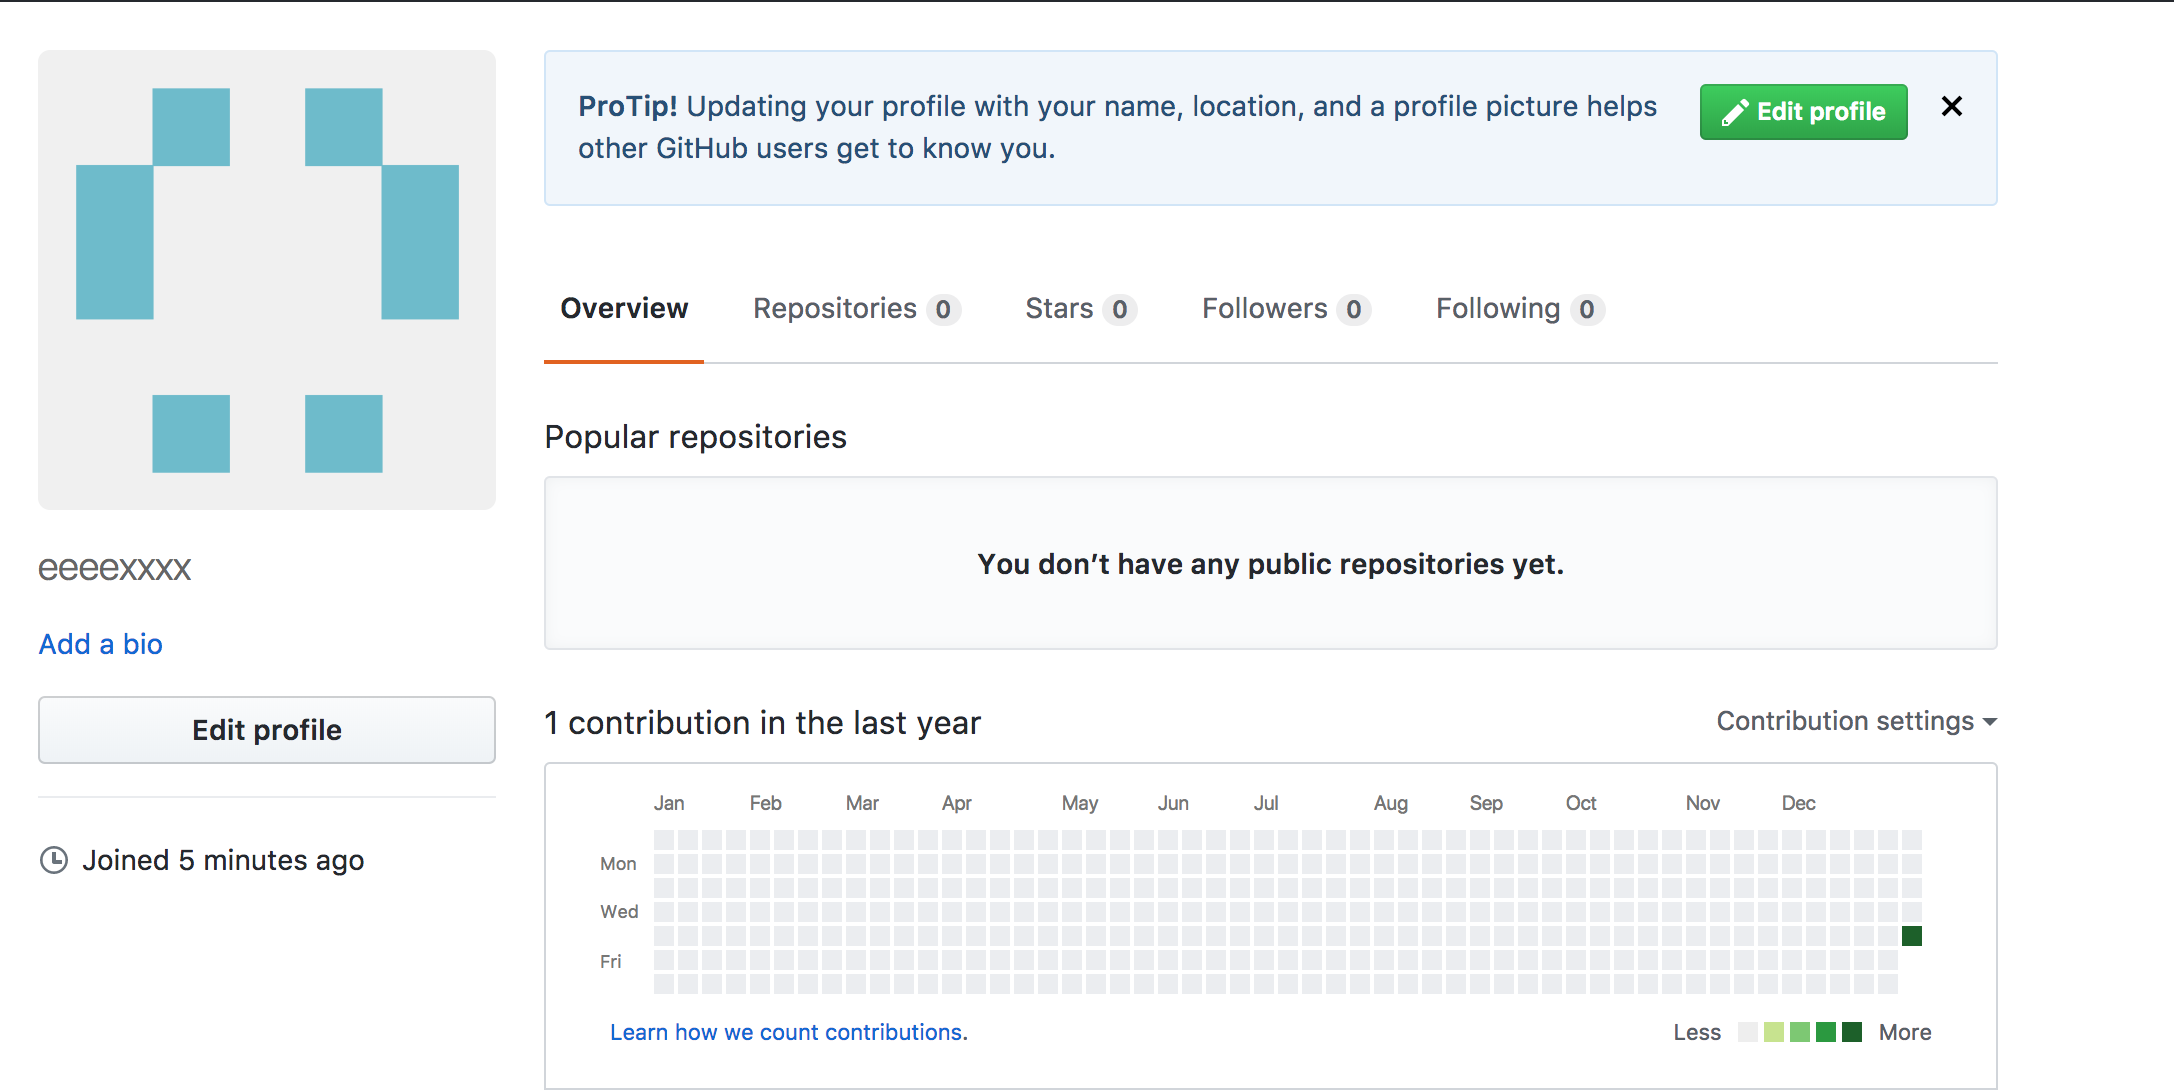
\includegraphics[width=.7\textwidth]{figures/init_profile.png}
\caption{Profile Screen}
\label{fig:init-prof}
\end{figure}

Click the ``Repositories" tab.
Click the button that says ``New" (see Figure \ref{fig:new-repo}).

\begin{figure}[h]
\centering
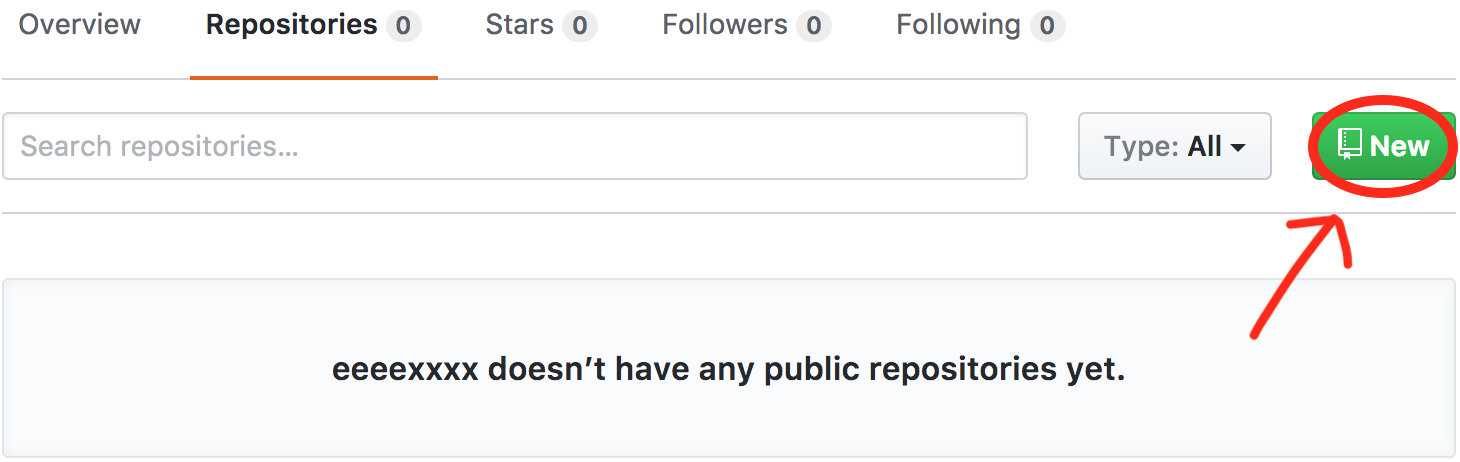
\includegraphics[width=.7\textwidth]{figures/new_repo.png}
\caption{New Repository}
\label{fig:new-repo}
\end{figure}

Name your repository.
It is customary to use dashes instead of underscores in repository names.
Make sure to initialize the repository with a README.md (see Figure \ref{fig:init-repo}).
If you accidentally forget to do this, that's okay; you can always add a README later.

\begin{figure}[h]
\centering
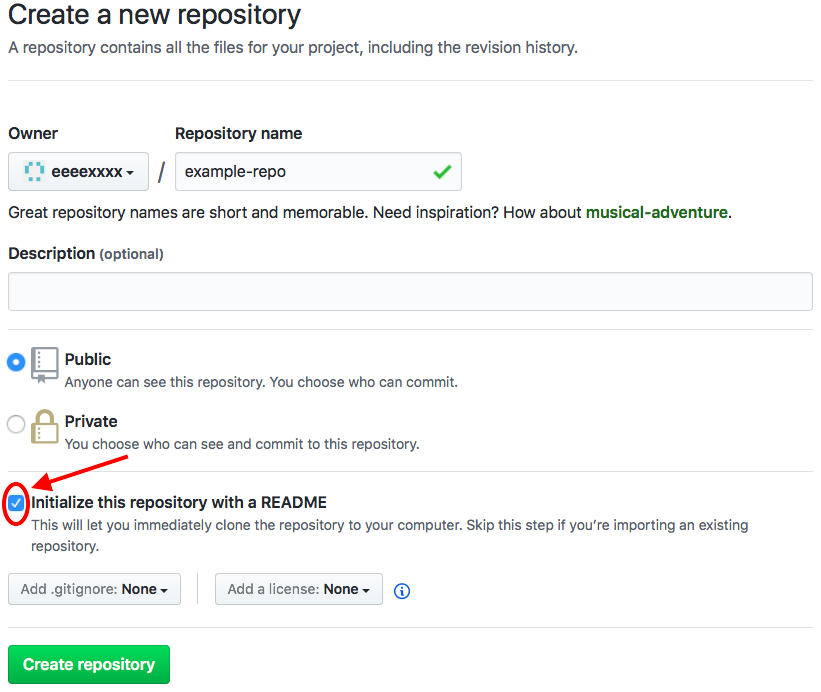
\includegraphics[width=.7\textwidth]{figures/init_repo.png}
\caption{Initialize the repository.}
\label{fig:init-repo}
\end{figure}

Click ``Create Repository" at the bottom of the page.
You should see a page that looks like Figure \ref{fig:repo-screen}.

\begin{figure}[h]
\centering
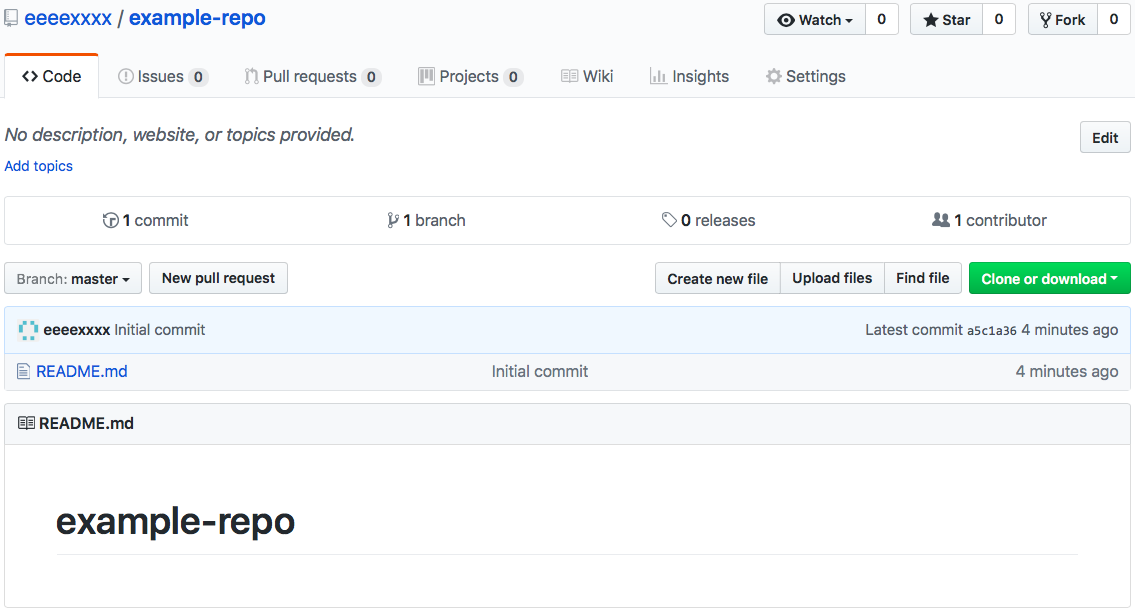
\includegraphics[width=.7\textwidth]{figures/repo_screen.png}
\caption{Repository screen.}
\label{fig:repo-screen}
\end{figure}

Congratulations!
You have just created your first GitHub repository.

\section*{Making Changes to Repositories}
There are a few ways to upload and change files in a GitHub repository.
The most common way to modify repositories is via the command line; see the next subsection for command line instructions.
It is highly, \textit{highly} recommended that you learn the command line to modify repositories.
The command line allows you to more freedom to modify your repositories and branches, and can streamline your workflow.
However, you can use the GitHub website to upload and download files to and from repositories.
You can also modify files using the website.
Note that you can't run Jupyter notebooks on the GitHub website, and when you try to edit Jupyter notebooks on the website, you have to comb through lots of nasty JSON lingo.
If you choose to use the website to make changes to the GitHub repository, you will have to download the Jupyter notebook, modify it on a local machine, and upload it back to the repository.
Instructions for using the website are in the subsection following the command line instructions.

If you do not have Git installed on your local machine, use the links below to download Git.
\begin{itemize}
\item[] Macs: \url{https://sourceforge.net/projects/git-osx-installer/files/}
\item[] Windows: \url{http://gitforwindows.org/}
\item[] Linux: In the Terminal, first type \texttt{sudo apt-get update} and hit Enter. Then type \texttt{sudo apt-get install git} and hit Enter.
\end{itemize} 

\subsection*{Using Command Line}
Let's walk through an example together.
In this example, we will configure Git on a local machine, clone the repository to a local machine, create a Jupyter notebook, add it to the repository, and push the changes.

First, set your username and email in Git.
Use the commands below to do this.

\begin{itemize}
\item[] \texttt{git config --global user.name "Your Name Here"}
\item[] \texttt{git config --global user.email "your\_email@website.com"}
\end{itemize}

Now Git is configured on your machine, and you are ready to clone the repository you made.
First, go to the repository screen on the GitHub website (Figure \ref{fig:repo-screen}).
Click the button that says ``Clone or download".
A drop-down window should appear that contains a link to your repository (see Figure \ref{fig:clone-screen}).
Copy the link in the drop-down window.

\begin{figure}[h]
\centering
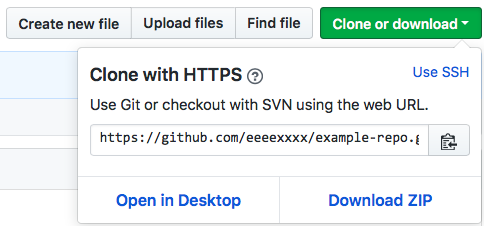
\includegraphics[width=.7\textwidth]{figures/clone_screen.png}
\caption{Jupyter notebook screen.}
\label{fig:clone-screen}
\end{figure}

Now open up your command line.
Navigate to the location where you want your repository to be (for example, I store all of my files on my desktop, so I would navigate to my desktop from my command line).
Once you have navigated to the location, type the following command: \texttt{git clone link\_to\_your\_repo}.
When your computer is done downloading the repository, you should see a folder with the name of your repository in the location where you wanted it.
Now you are ready to make some changes and push them to your master branch.

\subsubsection*{Making Changes}
For this example, we are going to make a Jupyter notebook and push it to the master branch.
In the command line, navigate to your repository, if you're not there already.
Type \texttt{jupyter notebook} and hit enter.
A web browser should open up with a page that looks like Figure \ref{fig:jupyter-dir}.
If a web browser did not automatically open, the command line should have provided a URL that you can copy and past directly into a browser to access the Jupyter notebook.

\begin{figure}[h]
\centering
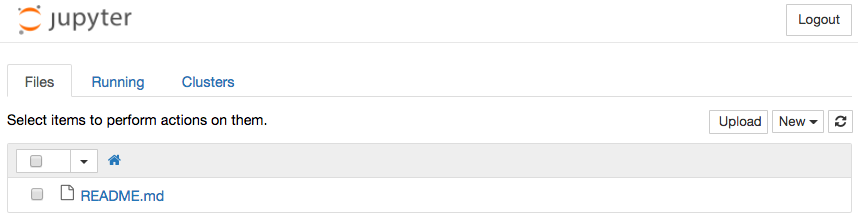
\includegraphics[width=.7\textwidth]{figures/jupyter_dir.png}
\caption{Jupyter notebook main screen.}
\label{fig:jupyter-dir}
\end{figure}

In the upper right-hand corner, click ``New".
A dropdown menu will appear.
Under the ``Notebooks" heading, click on Python 3 (see Figure \ref{fig:jupyter-dropdown}).
When you click ``Python 3", a new window will open in your browser with a screen that looks like Figure \ref{fig:jupyter}.

\begin{figure}[h]
\centering
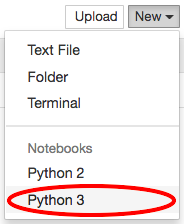
\includegraphics[width=.3\textwidth]{figures/jupyter_dropdown.png}
\caption{Create a Python 3 Jupyter notebook.}
\label{fig:jupyter-dropdown}
\end{figure}

\begin{figure}[h]
\centering
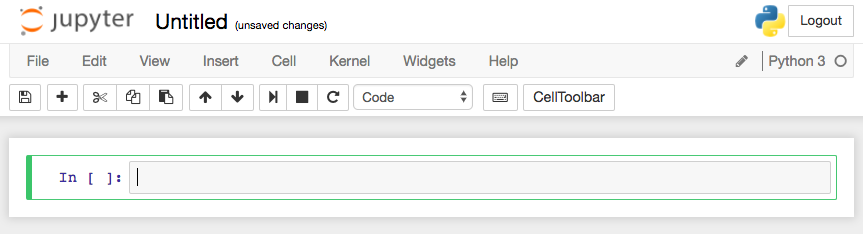
\includegraphics[width=.7\textwidth]{figures/jupyter.png}
\caption{A Jupyter notebook.}
\label{fig:jupyter}
\end{figure}

Change the name of the notebook from``Untitled" to ``example".
To do this, click the ``Untitled" text at the top of the notebook.
A window will appear; replace the ``Untitled" text with ``example".
See Figure \ref{fig:rename-notebook}.

\begin{figure}[h]
\centering
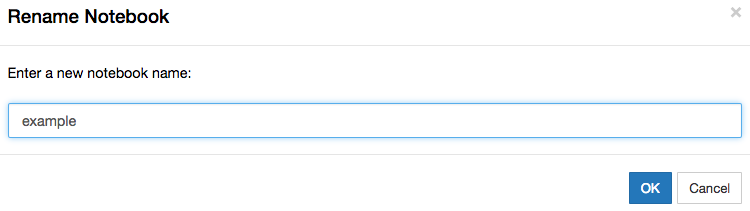
\includegraphics[width=.7\textwidth]{figures/rename_notebook.png}
\caption{Rename the notebook.}
\label{fig:rename-notebook}
\end{figure}

In the first cell, type \texttt{print("Hello World")}.
Then press Shift+Enter.
This key combination runs the cell.
A new cell will automatically appear below the cell with the print statement.
To save the notebook, hit Command+S.
Your notebook should now look like Figure \ref{fig:example-notebook}.

\begin{figure}[h]
\centering
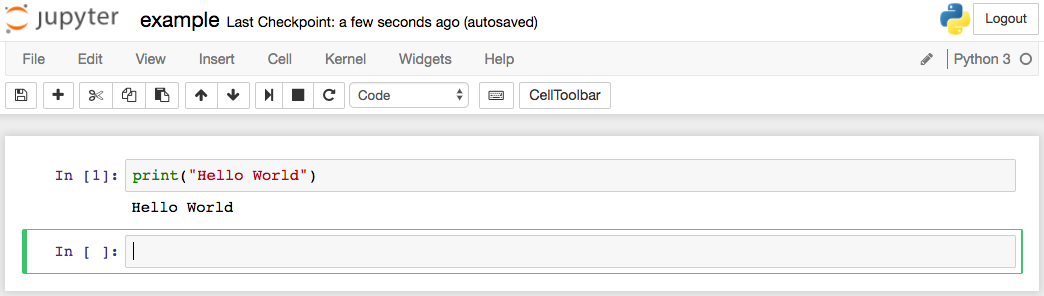
\includegraphics[width=.7\textwidth]{figures/example_notebook.png}
\caption{A Jupyter notebook.}
\label{fig:example-notebook}
\end{figure}

Now navigate to the command line where you launched Jupyter.
To stop the Jupyter server from running, hit Ctrl+c.
You will be prompted with the following message: \texttt{Shutdown this notebook server (y/[n])? }.
Type ``y" and hit enter.
This will shut down the Jupyter notebook.
If you didn't exit the browser window yet, it will look like Figure \ref{fig:jupyter-shutdown} after you shut down the Jupyter server.
You are safe to close all browser windows related to this Jupyter notebook.

\begin{figure}[h]
\centering
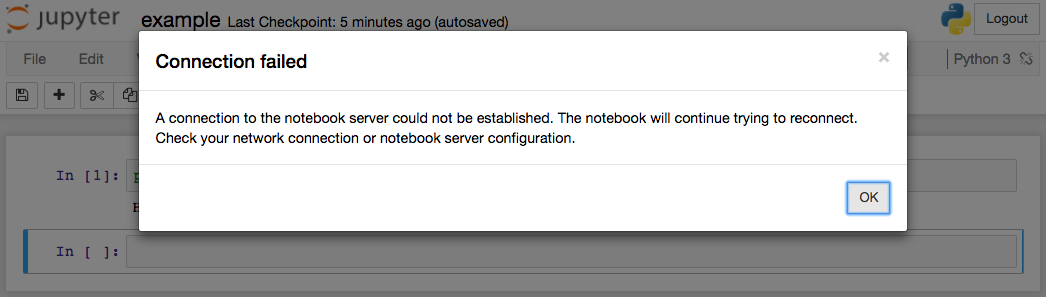
\includegraphics[width=.7\textwidth]{figures/jupyter_shutdown.png}
\caption{Shutting down a Jupyter notebook.}
\label{fig:jupyter-shutdown}
\end{figure}

\subsubsection*{Committing Changes}
In the command prompt, navigate to the repository, if you aren't already there.
Type \texttt{git status} and hit enter.
You should see a message that looks similar to Figure \ref{git-status}.

\begin{figure}[h]
\centering
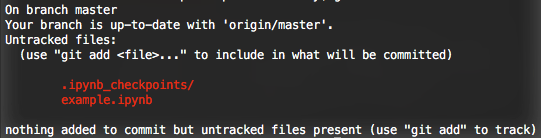
\includegraphics[width=.7\textwidth]{figures/git_status.png}
\caption{\texttt{git status}}
\label{fig:git-status}
\end{figure}

You want to add the notebook you just created to the Git index so Git knows to keep track of this file and any future changes made to it.
To do this, type \texttt{git add example.ipynb} and hit enter.
Now we are going to commit this change to the branch.
Then, type \texttt{git commit -m "example notebook"}.
A message that looks like Figure \ref{fig:git-commit} will appear.
Note that you can type any descriptive message you want in the quotes.
These messages are to help you keep track of the changes you make in each commit.
Now we want to push these changes up the master branch, so that any other machines with this repository can pull the changes you made.
Type \texttt{git push origin master} and hit enter.

\begin{figure}[h]
\centering
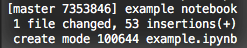
\includegraphics[width=.4\textwidth]{figures/git_commit.png}
\caption{\texttt{git commit}}
\label{fig:git-commit}
\end{figure}

\subsubsection*{Pulling Changes}

\subsubsection*{Pull Requests}

\subsection*{Using the Website}
\subsubsection*{Downloading Files}

\subsubsection*{Uploading Files}

\section*{Forking Repositories}
Navigate to the class repository. 
The link is \url{https://github.com/tfolkman/byu_econ_applied_machine_learning}.

\section*{Deleting Repositories}
PROCEED WITH CAUTION.
This action cannot be undone.

\end{document}
